\documentclass{standalone}
\usepackage{tikz}
\usetikzlibrary{patterns, positioning}

\begin{document}
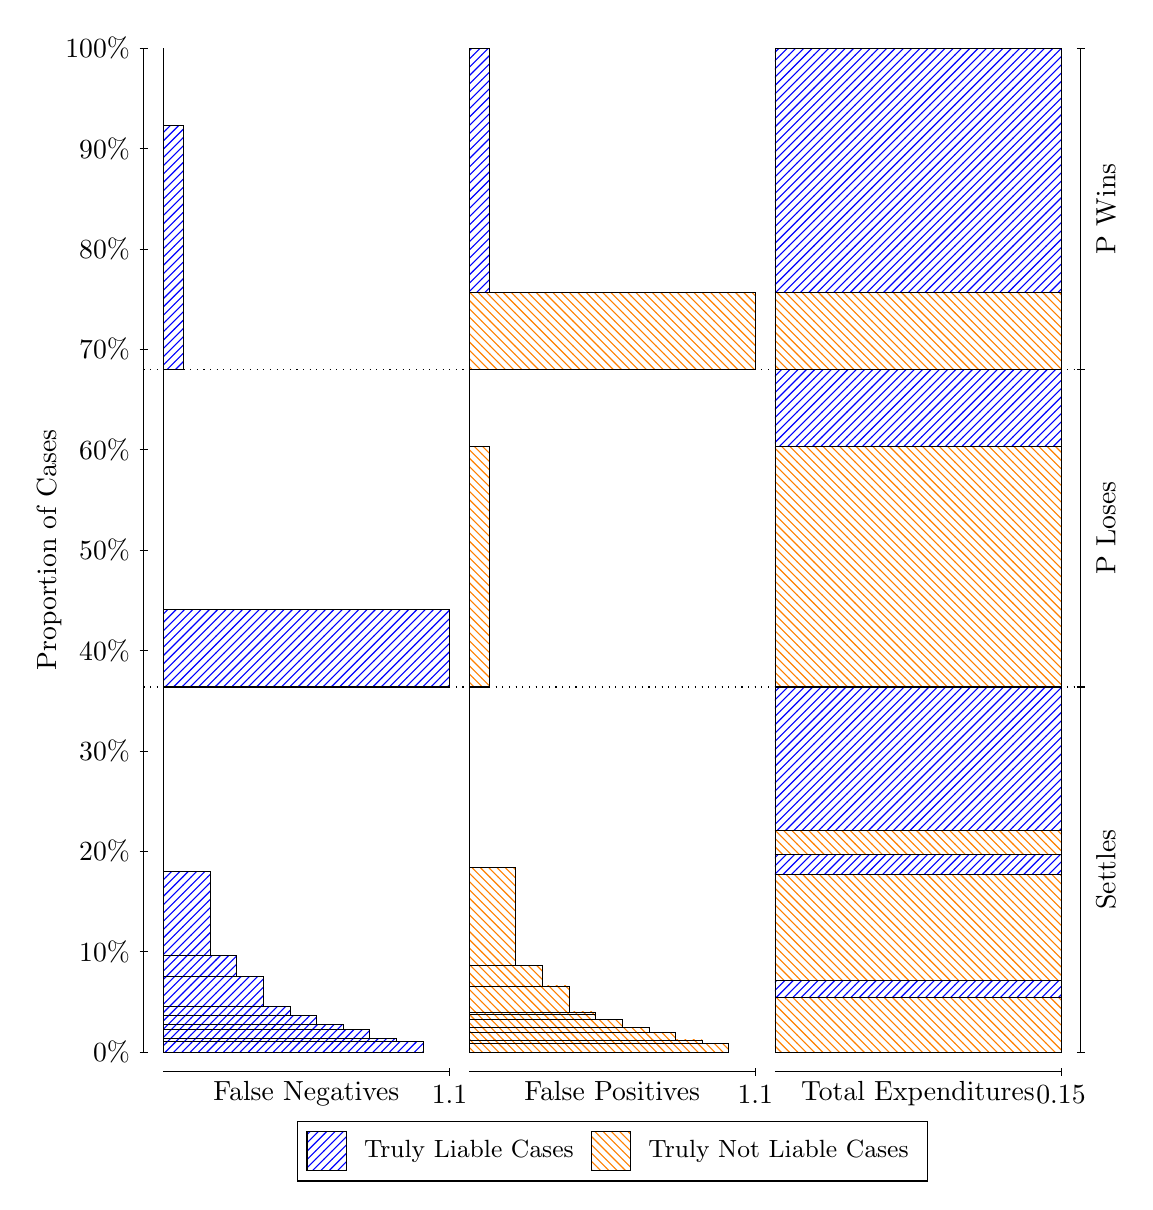
\begin{tikzpicture}
\draw[black, very thin] (1.5,1.75) -- (1.5,14.5);
\node[rotate=90, anchor=center] at (0.3, 8.125) {Proportion of Cases};
\draw[black, very thin] (1.45,1.75) -- (1.55,1.75);
\node[anchor=east] at (1.45, 1.75) {0\%};
\draw[black, very thin] (1.45,3.025) -- (1.55,3.025);
\node[anchor=east] at (1.45, 3.025) {10\%};
\draw[black, very thin] (1.45,4.3) -- (1.55,4.3);
\node[anchor=east] at (1.45, 4.3) {20\%};
\draw[black, very thin] (1.45,5.575) -- (1.55,5.575);
\node[anchor=east] at (1.45, 5.575) {30\%};
\draw[black, very thin] (1.45,6.85) -- (1.55,6.85);
\node[anchor=east] at (1.45, 6.85) {40\%};
\draw[black, very thin] (1.45,8.125) -- (1.55,8.125);
\node[anchor=east] at (1.45, 8.125) {50\%};
\draw[black, very thin] (1.45,9.4) -- (1.55,9.4);
\node[anchor=east] at (1.45, 9.4) {60\%};
\draw[black, very thin] (1.45,10.675) -- (1.55,10.675);
\node[anchor=east] at (1.45, 10.675) {70\%};
\draw[black, very thin] (1.45,11.95) -- (1.55,11.95);
\node[anchor=east] at (1.45, 11.95) {80\%};
\draw[black, very thin] (1.45,13.225) -- (1.55,13.225);
\node[anchor=east] at (1.45, 13.225) {90\%};
\draw[black, very thin] (1.45,14.5) -- (1.55,14.5);
\node[anchor=east] at (1.45, 14.5) {100\%};

\draw[black, very thin] (13.4,1.75) -- (13.4,14.5);
\draw[black, very thin] (13.35,1.75) -- (13.45,1.75);
\node[anchor=west] at (13.35, 1.75) {};
\draw[black, very thin] (13.35,6.3856) -- (13.45,6.3856);
\node[anchor=west] at (13.35, 6.3856) {};
\draw[black, very thin] (13.35,6.3892) -- (13.45,6.3892);
\node[anchor=west] at (13.35, 6.3892) {};
\draw[black, very thin] (13.35,10.415) -- (13.45,10.415);
\node[anchor=west] at (13.35, 10.415) {};
\draw[black, very thin] (13.35,14.5) -- (13.45,14.5);
\node[anchor=west] at (13.35, 14.5) {};

\draw[black, very thin, pattern color=blue, pattern=north east lines] (1.75,1.75) rectangle (5.0453,1.8822);
\draw[black, very thin, pattern color=blue, pattern=north east lines] (1.75,1.8822) rectangle (4.7074,1.9255);
\draw[black, very thin, pattern color=blue, pattern=north east lines] (1.75,1.9255) rectangle (4.3694,2.0335);
\draw[black, very thin, pattern color=blue, pattern=north east lines] (1.75,2.0335) rectangle (4.0314,2.0977);
\draw[black, very thin, pattern color=blue, pattern=north east lines] (1.75,2.0977) rectangle (3.6934,2.2189);
\draw[black, very thin, pattern color=blue, pattern=north east lines] (1.75,2.2189) rectangle (3.3554,2.3321);
\draw[black, very thin, pattern color=blue, pattern=north east lines] (1.75,2.3321) rectangle (3.0174,2.709);
\draw[black, very thin, pattern color=blue, pattern=north east lines] (1.75,2.709) rectangle (2.6795,2.9786);
\draw[black, very thin, pattern color=blue, pattern=north east lines] (1.75,2.9786) rectangle (2.3415,4.0405);
\draw[black, very thin, pattern color=orange, pattern=north west lines] (1.75,4.0405) rectangle (1.75,6.3856);
\draw[black, very thin, pattern color=blue, pattern=north east lines] (1.75,6.3856) rectangle (5.3833,6.386);
\draw[black, very thin, pattern color=orange, pattern=north west lines] (1.75,6.386) rectangle (1.75,6.3892);
\draw[black, very thin, pattern color=blue, pattern=north east lines] (1.75,6.3892) rectangle (5.3833,7.3674);
\draw[black, very thin, pattern color=orange, pattern=north west lines] (1.75,7.3674) rectangle (1.75,10.415);
\draw[black, very thin, pattern color=blue, pattern=north east lines] (1.75,10.415) rectangle (2.0035,13.521);
\draw[black, very thin, pattern color=orange, pattern=north west lines] (1.75,13.521) rectangle (1.75,14.5);
\draw[black, very thin, pattern color=orange, pattern=north west lines] (5.6333,1.75) rectangle (8.9287,1.8604);
\draw[black, very thin, pattern color=orange, pattern=north west lines] (5.6333,1.8604) rectangle (8.5907,1.9038);
\draw[black, very thin, pattern color=orange, pattern=north west lines] (5.6333,1.9038) rectangle (8.2527,2.0032);
\draw[black, very thin, pattern color=orange, pattern=north west lines] (5.6333,2.0032) rectangle (7.9147,2.0591);
\draw[black, very thin, pattern color=orange, pattern=north west lines] (5.6333,2.0591) rectangle (7.5767,2.1607);
\draw[black, very thin, pattern color=orange, pattern=north west lines] (5.6333,2.1607) rectangle (7.2388,2.2238);
\draw[black, very thin, pattern color=orange, pattern=north west lines] (5.6333,2.2238) rectangle (7.2388,2.2586);
\draw[black, very thin, pattern color=orange, pattern=north west lines] (5.6333,2.2586) rectangle (6.9008,2.5882);
\draw[black, very thin, pattern color=orange, pattern=north west lines] (5.6333,2.5882) rectangle (6.5628,2.8504);
\draw[black, very thin, pattern color=orange, pattern=north west lines] (5.6333,2.8504) rectangle (6.2248,4.0952);
\draw[black, very thin, pattern color=blue, pattern=north east lines] (5.6333,4.0952) rectangle (5.6333,6.3856);
\draw[black, very thin, pattern color=orange, pattern=north west lines] (5.6333,6.3856) rectangle (5.8868,6.3889);
\draw[black, very thin, pattern color=blue, pattern=north east lines] (5.6333,6.3889) rectangle (5.6333,6.3892);
\draw[black, very thin, pattern color=orange, pattern=north west lines] (5.6333,6.3892) rectangle (5.8868,9.4373);
\draw[black, very thin, pattern color=blue, pattern=north east lines] (5.6333,9.4373) rectangle (5.6333,10.415);
\draw[black, very thin, pattern color=orange, pattern=north west lines] (5.6333,10.415) rectangle (9.2667,11.394);
\draw[black, very thin, pattern color=blue, pattern=north east lines] (5.6333,11.394) rectangle (5.8868,14.5);
\draw[black, very thin, pattern color=orange, pattern=north west lines] (9.5167,1.75) rectangle (13.15,2.4396);
\draw[black, very thin, pattern color=blue, pattern=north east lines] (9.5167,2.4396) rectangle (13.15,2.6551);
\draw[black, very thin, pattern color=orange, pattern=north west lines] (9.5167,2.6551) rectangle (13.15,4.0016);
\draw[black, very thin, pattern color=blue, pattern=north east lines] (9.5167,4.0016) rectangle (13.15,4.2549);
\draw[black, very thin, pattern color=orange, pattern=north west lines] (9.5167,4.2549) rectangle (13.15,4.564);
\draw[black, very thin, pattern color=blue, pattern=north east lines] (9.5167,4.564) rectangle (13.15,6.3856);
\draw[black, very thin, pattern color=orange, pattern=north west lines] (9.5167,6.3856) rectangle (13.15,6.3889);
\draw[black, very thin, pattern color=blue, pattern=north east lines] (9.5167,6.3889) rectangle (13.15,6.3892);
\draw[black, very thin, pattern color=orange, pattern=north west lines] (9.5167,6.3892) rectangle (13.15,9.4373);
\draw[black, very thin, pattern color=blue, pattern=north east lines] (9.5167,9.4373) rectangle (13.15,10.415);
\draw[black, very thin, pattern color=orange, pattern=north west lines] (9.5167,10.415) rectangle (13.15,11.394);
\draw[black, very thin, pattern color=blue, pattern=north east lines] (9.5167,11.394) rectangle (13.15,14.5);
\draw[black, dotted] (1.5,6.3856) -- (13.4,6.3856);
\draw[black, dotted] (1.5,6.3892) -- (13.4,6.3892);
\draw[black, dotted] (1.5,10.415) -- (13.4,10.415);
\draw[black, very thin] (1.75,1.5) -- (5.3833,1.5);
\node[anchor=north] at (3.5667, 1.5) {False Negatives};
\draw[black, very thin] (5.3833,1.45) -- (5.3833,1.55);
\node[anchor=north] at (5.3833, 1.45) {1.1};

\draw[black, very thin] (5.6333,1.5) -- (9.2667,1.5);
\node[anchor=north] at (7.45, 1.5) {False Positives};
\draw[black, very thin] (9.2667,1.45) -- (9.2667,1.55);
\node[anchor=north] at (9.2667, 1.45) {1.1};

\draw[black, very thin] (9.5167,1.5) -- (13.15,1.5);
\node[anchor=north] at (11.333, 1.5) {Total Expenditures};
\draw[black, very thin] (13.15,1.45) -- (13.15,1.55);
\node[anchor=north] at (13.15, 1.45) {0.15};

\node[black, centered, rotate=90] at (13.72, 4.0678) {Settles};

\node[black, centered, rotate=90] at (13.72, 8.4023) {P Loses};
\node[black, centered, rotate=90] at (13.72, 12.458) {P Wins};

\draw (7.449999999999999,1.5) node[draw=none] (baseCoordinate) {};
\begin{scope}[align=center]
        \matrix[scale=0.5, draw=black, below=0.5cm of baseCoordinate, nodes={draw}, column sep=0.1cm]{
            \node[rectangle, draw, minimum width=0.5cm, minimum height=0.5cm, pattern=north east lines, pattern color=blue] {}; &
            \node[draw=none, font=\small] (B) {Truly Liable Cases}; &
            \node[rectangle, draw, minimum width=0.5cm, minimum height=0.5cm, pattern=north west lines, pattern color=orange] {}; &
            \node[draw=none, font=\small] (B) {Truly Not Liable Cases}; \\
            };
\end{scope}

\end{tikzpicture}
\end{document}